%%
% This is an Overleaf template for presentations
% using the TUM Corporate Desing https://www.tum.de/cd
%
% For further details on how to use the template, take a look at our
% GitLab repository and browse through our test documents
% https://gitlab.lrz.de/latex4ei/tum-templates.
%
% The tumbeamer class is based on the beamer class.
% If you need further customization please consult the beamer class guide
% https://ctan.org/pkg/beamer.
% Additional class options are passed down to the base class.
%%


\documentclass[
  english,            % define the document language (english, german)
  aspectratio=169,    % define the aspect ratio (169, 43)
  % handout=2on1,       % create handout with multiple slides (2on1, 4on1)
  % partpage=false,     % insert page at beginning of parts (true, false)
  sectionpage=false,   % insert page at beginning of sections (true, false)
]{tumbeamer}

% load additional packages
\usepackage{booktabs}

\usepackage{siunitx}
\usepackage{makecell}
\usepackage{multirow}

%TODO: change font
\usepackage[sc]{mathpazo}

\usepackage[%
    style=phys,%
    autocite=plain,%
    articletitle=false,biblabel=brackets,%
    chaptertitle=false,pageranges=false%
]
{biblatex}

\bibliography{bibliography}

% hide "(visited on ...)" access dates in citations
\AtEveryCitekey{\clearfield{urlyear}\clearfield{urlmonth}\clearfield{urlday}}
\AtEveryBibitem{\clearfield{urlyear}\clearfield{urlmonth}\clearfield{urlday}}


\newcommand\blfootnote[1]{%
  \begingroup
  \renewcommand\thefootnote{}\footnote{#1}%
  \addtocounter{footnote}{-1}%
  \endgroup
}

\usepackage[beamer,customcolors]{hf-tikz}

\tikzset{hl/.style={
    set fill color=green!80!black!20,
    set border color=green!80!black,
  },
}

\tikzset{iv/.style={
    set fill color=white!00,
    set border color=green!00,
  },
}

\usetikzlibrary{arrows.meta}

% .:: Title page diagram
% ----------------------------------------------------------------------------
% "TUM diagram" title page style: the "TUM tower" layout, with the tower image
% replaced by the TikZ drawing in figures/title_diagram.tex.

\definecolor{TitleLightBlue}{HTML}{B7CCE2}
\definecolor{TitleDarkBlue}{HTML}{8FA6C9}
\definecolor{TitleOlive}{HTML}{CDD394}
\definecolor{TitleOrange}{HTML}{E9B695}
\definecolor{TitleRed}{HTML}{DD9C9C}

\makeatletter
\defbeamertemplate{background}{TUM diagram}{
  \begin{tikzpicture}[remember picture, overlay]
    \node[anchor=north east, inner sep=0, outer sep=0]
      at (\paperwidth-\@tum@hmargin@, -\@tum@vmargin@)
      {\theTUMLogo[height=\@tum@logoheight@, color=\@tum@logocolor@]};
    \node[anchor=south east, inner sep=0, outer sep=0]
      at (\paperwidth-\@tum@hmargin@, -\paperheight+\@tum@vmargin@)
      {\resizebox{!}{0.62\paperheight}{% Title-page diagram: recommender-system challenges around sustainability.
% Drawn with TikZ and \input by the title page background in settings.tex.
% Symmetric around the origin: \sx/\sy place the side and top/bottom ellipses.
\begin{tikzpicture}[scale=1.35,
    challenge/.style={draw=black, line width=0.4pt, fill opacity=0.75, text opacity=1},
    caption/.style={anchor=center, inner sep=2pt, font=\sffamily\fontsize{16}{19}\selectfont, text=black},
  ]
  \def\sx{2.35}  % horizontal offset of the side ellipses
  \def\sy{2.35}  % vertical offset of the top and bottom ellipses

  % side ellipses
  \draw[challenge, fill=TitleOlive]  (-\sx,0) ellipse (0.95 and 2.55);
  \draw[challenge, fill=TitleOrange] ( \sx,0) ellipse (0.95 and 2.55);
  % top and bottom ellipses
  \draw[challenge, fill=TitleLightBlue] (0, \sy) ellipse (2.35 and 0.68);
  \draw[challenge, fill=TitleDarkBlue]  (0,-\sy) ellipse (2.35 and 0.68);
  % centre
  \draw[fill=TitleRed, draw=red!80!black, dashed, line width=0.8pt] (0,0) circle (1.30);

  \node[caption] at (0, \sy) {Cold-start};
  \node[caption] at (-\sx,0) {Sparsity};
  \node[caption] at ( \sx,0) {Accuracy};
  \node[caption] at (0,-\sy) {Scalability};
  \node[caption] at (0,0)    {Sustainability};
\end{tikzpicture}
}};
  \end{tikzpicture}
}[action]{
  \pgfmathparse{.5\textwidth*\pgfkeysvalueof{/TUM/beamer/setup/tower scale}}
  \setlength{\@tum@towerwidth@}{\pgfmathresult pt}
  \if@tum@widescreen@
    \setlength{\@tum@titlewidth@}{.8\textwidth}
    \setlength{\@tum@authorwidth@}{\textwidth-\@tum@towerwidth@}
  \else
    \setlength{\@tum@titlewidth@}{\textwidth}
    \setlength{\@tum@authorwidth@}{\textwidth-.9\@tum@towerwidth@}
  \fi
}

\pgfqkeys{/TUM/beamer/setup/title page}{
  TUM diagram/.code = {
      \setTUMframestyle{title page}{
        \setbeamertemplate{background canvas}[TUM default]
        \setbeamertemplate{background}[TUM diagram]
        \setbeamertemplate{title page}[TUM default]
      }
    },
}
\makeatother


% macro to configure the style of the presentation
\TUMbeamersetup{
  title page = TUM diagram,       % style of the title page
  part page = TUM toc,            % style of part pages
  section page = TUM toc,         % style of section pages
  content page = TUM more space,  % style of normal content pages
  tower scale = 1.15,              % scaling factor of TUM tower (if used)
  headline = TUM empty,      % which variation of headline to use
  footline = TUM empty,         % which variation of footline to use
  % configure on which pages headlines and footlines should be printed
  headline on = {title page},
  footline on = {title page=false},
}


\graphicspath{
    {figures/}
    {logos/}
}




% presentation metadata
\title[Energy-Aware Hybrid Recommender Systems]{Energy-Aware Hybrid\\Recommender Systems\\Across the User Lifecycle}
\subtitle{}
\author{\theAuthorName}

\institute{\theChairName\\\theDepartmentName\\\theUniversityName}
\date{\today} % TODO: set presentation date

\footline{\insertauthor~|~\insertshorttitle~|~\insertshortdate}


\begin{document}

\maketitle

% !TeX root = ../main.tex
% Add the above to each file to make compiling the PDF easier in some editors.

\section{Introduction and Background}


\begin{frame}{Introduction}
    \setbeamercovered{transparent}
  \begin{columns}
      \begin{column}{0.65\textwidth}
          \vspace{4mm}
          \begin{itemize}
              \large
        \setlength\itemsep{1.5em}
            \item<1-> Recommender models are becoming more expensive without proportionate gains in quality\footnotemark
            \item<2-> A recommender is not trained once: new users arrive and preferences shift, so the model must be kept up to date
            \item<3-> The recurring carbon cost of keeping it current has not been measured
          \end{itemize}
      \end{column}
      \begin{column}{0.35\textwidth}
          \vspace{-4mm}
          \begin{center}
          \onslide<2->{%
          \begin{tikzpicture}[>=Stealth, box/.style={draw=TUMBlue, thick, rounded corners, minimum width=26mm, minimum height=8mm, align=center}]
              \node[box, fill=TUMBlue!15] (t) at (0,0) {Train};
              \node[box] (d) at (0,-1.5) {Deploy};
              \node[box] (s) at (0,-3.0) {New interactions};
              \node[box, draw=TUMOrange, fill=TUMOrange!15] (u) at (0,-4.5) {Update?};
              \draw[->, thick] (t) -- (d);
              \draw[->, thick] (d) -- (s);
              \draw[->, thick] (s) -- (u);
              \draw[->, thick] (u.east) -- ++(0.6,0) |- (d.east);
          \end{tikzpicture}}
          \end{center}
      \end{column}
  \end{columns}
\footnotetext[1]<1->{\fullcite{spillo2023sustainability}\\\fullcite{vente2024clicks}}
\end{frame}

\begin{frame}{Central Research Question}
    \vspace*{\fill}
    \begin{center}
        \huge What does it cost to keep a recommender up to date, and can a cheaper hybrid mechanism deliver comparable quality?
    \end{center}
\end{frame}

% !TeX root = ../main.tex
% Add the above to each file to make compiling the PDF easier in some editors.

\begin{frame}{LightGCN}
    \large
    \begin{columns}
    \begin{column}{0.5\linewidth}
        \vspace{5mm}
        \begin{center}
        \begin{tikzpicture}[
            u/.style={circle,draw=TUMBlue,fill=TUMBlue!15,thick,minimum size=7mm},
            i/.style={rectangle,draw=TUMOrange,fill=TUMOrange!15,thick,minimum size=6mm}]
            \node[u] (u1) at (0,2) {$u_1$};
            \node[u] (u2) at (0,1) {$u_2$};
            \node[u] (u3) at (0,0) {$u_3$};
            \node[i] (i1) at (2.5,2.3) {$i_1$};
            \node[i] (i2) at (2.5,1.5) {$i_2$};
            \node[i] (i3) at (2.5,0.7) {$i_3$};
            \node[i] (i4) at (2.5,-0.1) {$i_4$};
            \draw[thick] (u1)--(i1) (u1)--(i2) (u2)--(i2) (u2)--(i3) (u3)--(i3) (u3)--(i4);
        \end{tikzpicture}
        \end{center}
        \begin{center}
            User--Item Interaction Graph
        \end{center}
    \end{column}
    \begin{column}{0.5\linewidth}
        \vspace{10mm}
        \begin{center}
            Neighborhood aggregation:
        \end{center}
        \[
            \mathbf{e}_u^{(k)} = \sum_{i \in \mathcal{N}_u} \frac{1}{\sqrt{|\mathcal{N}_u|}\sqrt{|\mathcal{N}_i|}} \mathbf{e}_i^{(k-1)}
        \]
        \vspace{3mm}
        \begin{center}
            Prediction: $\hat{y}_{ui} = \mathbf{e}_u^\top \mathbf{e}_i$\\
        \end{center}
    \end{column}
    \begin{column}{0.1\linewidth}
    \end{column}
    \end{columns}
    \slidecite{lightgcn}{He et al., SIGIR 2020}
\end{frame}


\begin{frame}{Measuring Carbon Emissions}
    \setbeamercovered{transparent}
    \large
    \begin{columns}
    \begin{column}{0.4\linewidth}
        \vspace{8mm}
        \begin{center}
            CPU and RAM energy estimated\\with CodeCarbon
        \end{center}
    \end{column}
    \begin{column}{0.5\linewidth}
        \vspace{11mm}
        \begin{align*}
            &\uncover<2->{\text{emissions} = C \cdot E} \\[5mm]
            &\uncover<3->{C = \sum_{s \in S} e_s \cdot p_s} \\[3mm]
            &\uncover<3->{C\ \text{(Germany)} = 381\ \text{\small g\,CO$_2$eq/kWh}}
        \end{align*}
    \end{column}
    \begin{column}{0.1\linewidth}
    \end{column}
    \end{columns}
    \slidecite{codecarbon-methodology}{CodeCarbon, Methodology, 2024}
\end{frame}


\begin{frame}{Evaluation Metrics}
    \setbeamercovered{transparent}
    \large
    \begin{columns}
    \begin{column}{0.4\linewidth}
        \vspace{10mm}
        \begin{center}
            Per batch: score all items,\\mask items already seen,\\recommend the top 10\\
            \vspace{5mm}
            Relevant: items the user\\liked in this batch
        \end{center}
    \end{column}
    \begin{column}{0.5\linewidth}
        \pause
        \begin{align*}
            &\text{Precision@}10 = \frac{\text{relevant items retrieved}}{\text{10}} \\[9mm]
            \pause
            &\text{Recall@}10 = \frac{\text{relevant items retrieved}}{\text{relevant items}} \\[9mm]
            \pause
            &\text{NDCG@}10 = \frac{\text{hits, weighted by rank}}{\text{best possible ranking}}
        \end{align*}
    \end{column}
    \begin{column}{0.1\linewidth}
    \end{column}
    \end{columns}
\end{frame}


\begin{frame}{Content Signals: Location and Category}
    \begin{columns}
    \begin{column}{0.5\linewidth}
        \begin{figure}[h]
            \centering
            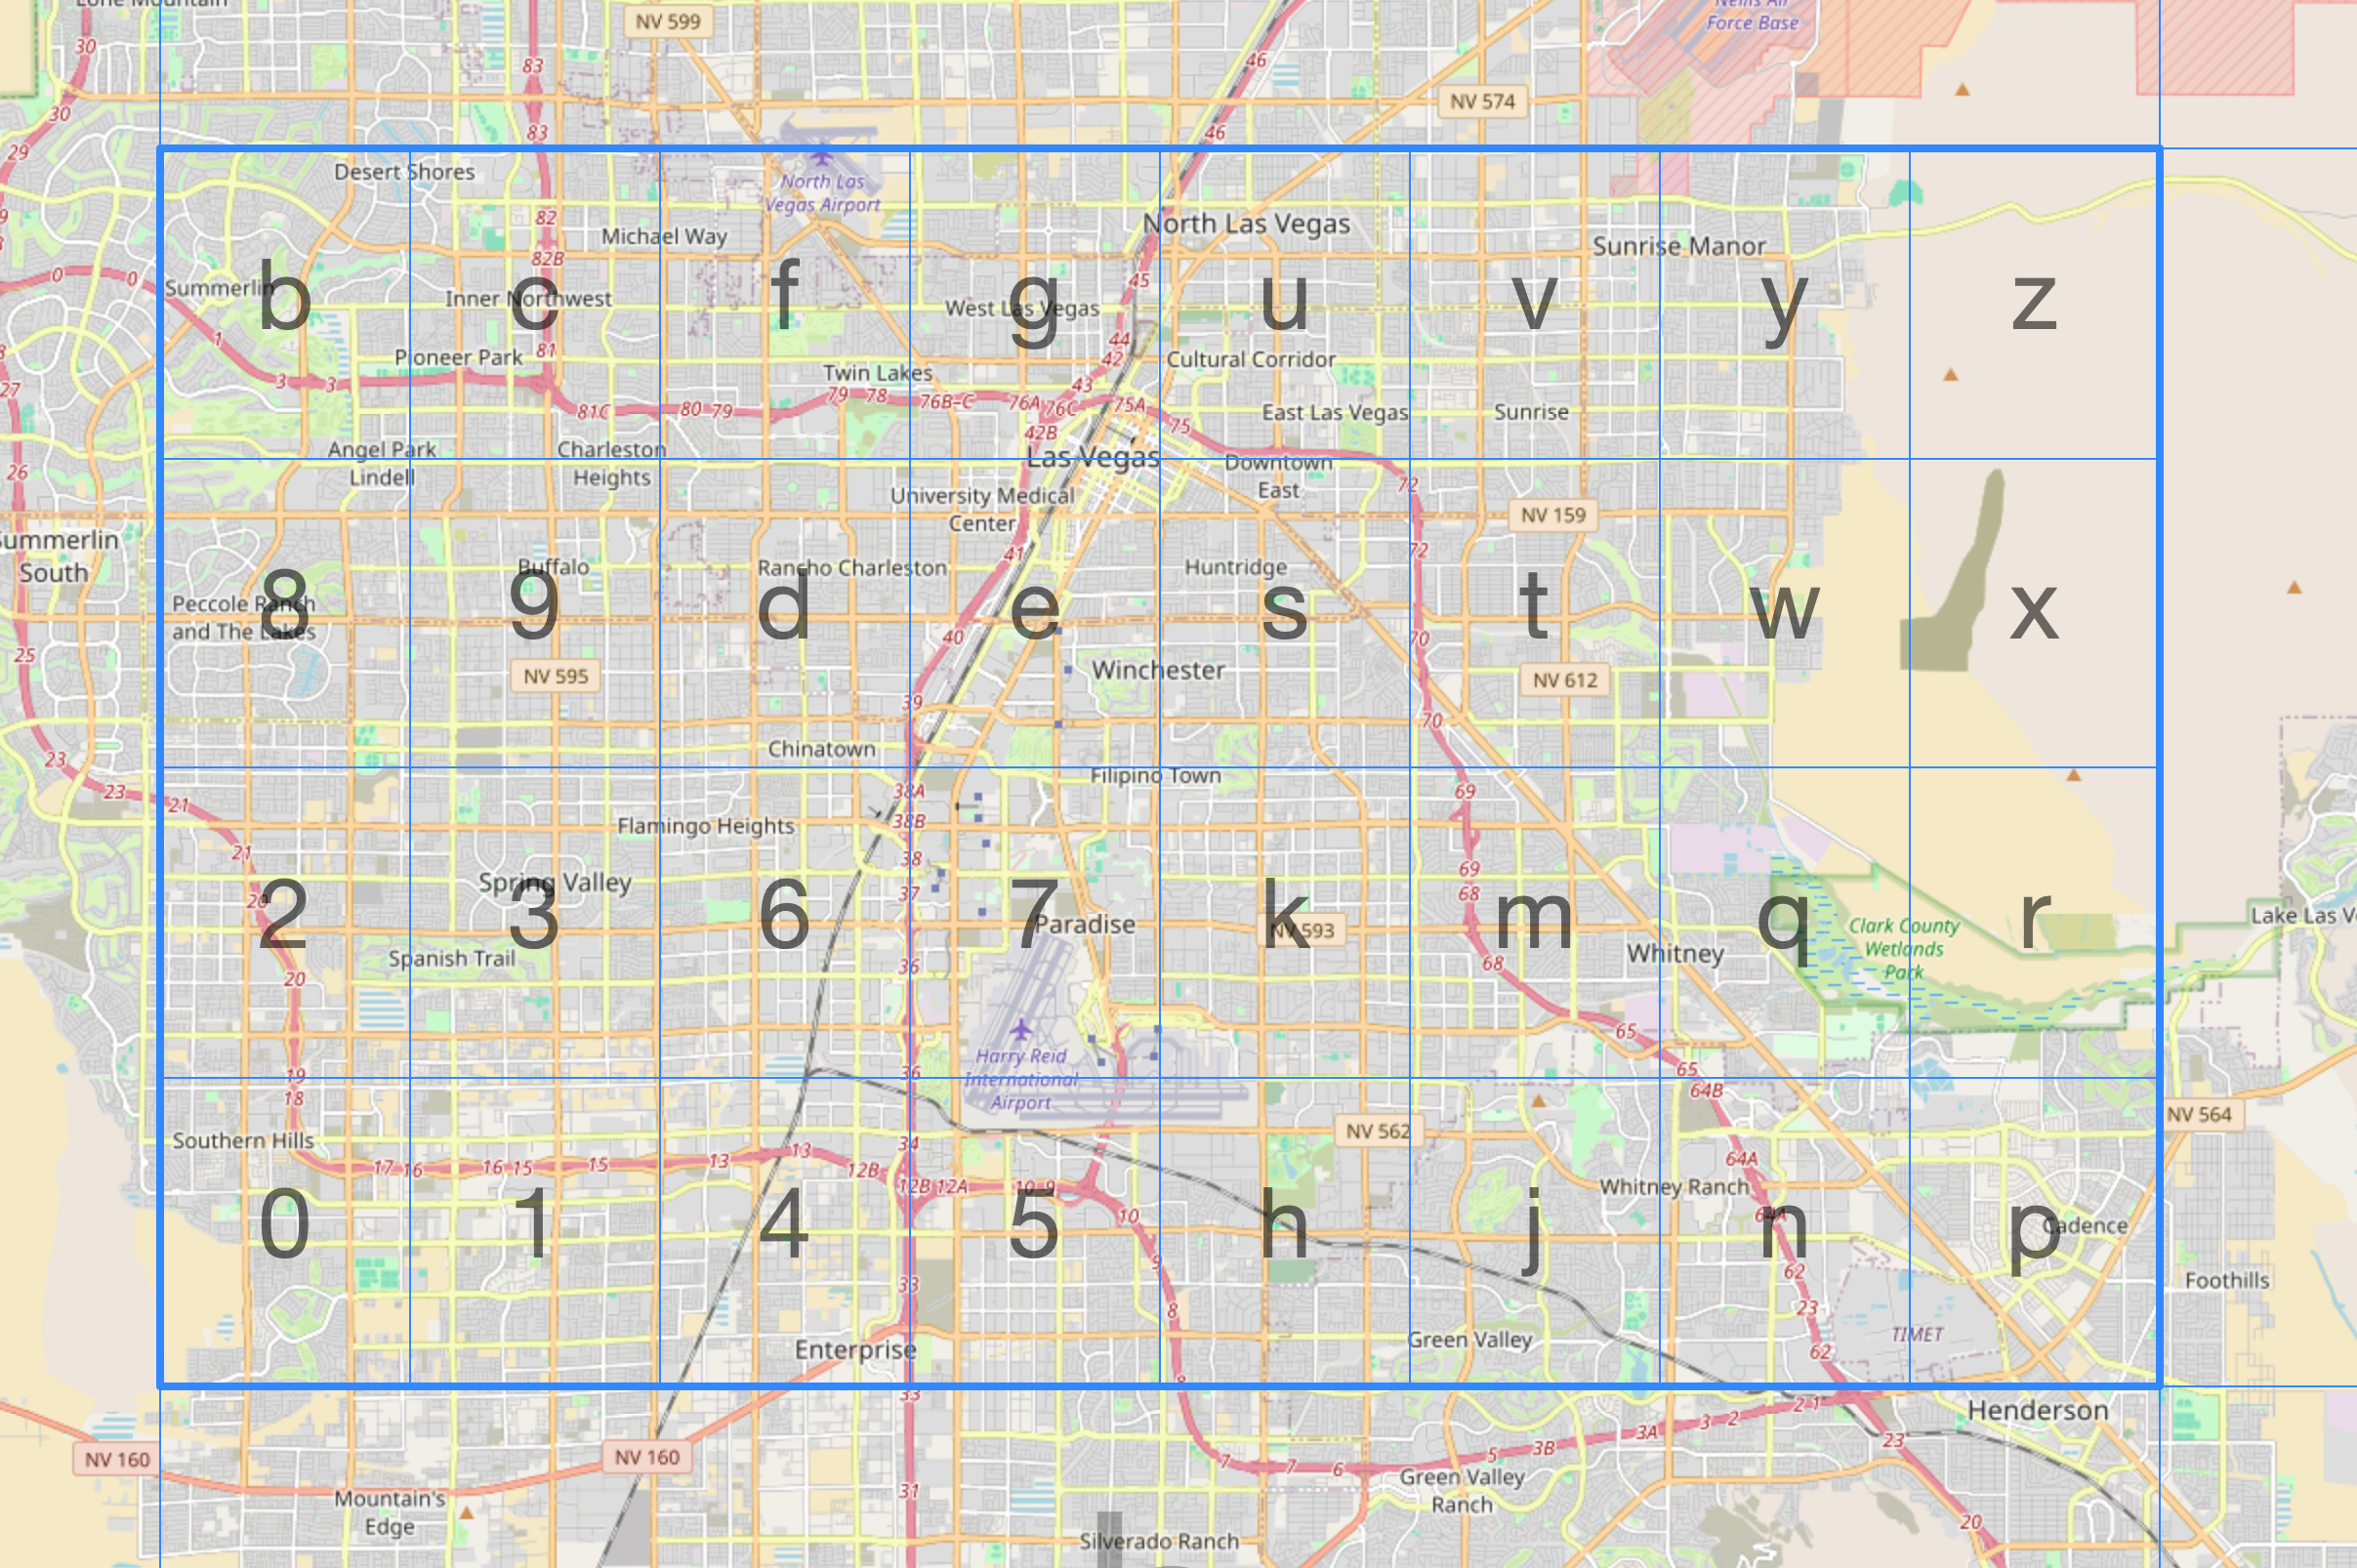
\includegraphics[width=0.9\linewidth]{geohash.png}
        \end{figure}
    \end{column}
    \begin{column}{0.45\linewidth}
        \begin{itemize}
            \large
            \setlength\itemsep{1.5em}
            \item \textbf{Location:} geohash cells, nearby businesses share a prefix
            \item \textbf{Category:} business category
            \item MovieLens: genre and release decade instead
        \end{itemize}
    \end{column}
    \end{columns}
    \slidecite{niemeyer2008geohash,geohash-softeng}{Niemeyer, geohash.org, 2008 \textperiodcentered{} Figure: Geohash Explorer, geohash.softeng.co}
\end{frame}


\begin{frame}{Content-Based Initialization}
    \vspace{2mm}
    \begin{center}
    \resizebox{0.98\textwidth}{!}{%
    \begin{tikzpicture}[
        >=Stealth,
        cell/.style={draw=TUMGray, minimum size=5mm, inner sep=0pt, font=\scriptsize},
        lbl/.style={font=\small},
        stage/.style={font=\bfseries, text=TUMBlue, anchor=center},
    ]

    % ---------------- 1: profiles of trained users ----------------
    \node[stage] at (1.4,3.3) {1\;\; Profile trained users};
    \foreach \b in {1,...,4} {
        \node[lbl, font=\scriptsize] at (0.25+0.5*\b,2.3) {$g_{\b}$};
    }
    \foreach \u/\row in {1/{3,0,1,0},2/{0,2,0,1},3/{1,0,4,0},4/{0,0,1,2}} {
        \node[lbl] at (0.1,2.25-0.5*\u) {$u_{\u}$};
        \foreach \v [count=\b] in \row {
            \pgfmathtruncatemacro{\shade}{min(\v*20,80)}
            \ifnum\shade>50 \node[cell, fill=TUMBlue!\shade, text=white] at (0.25+0.5*\b,2.25-0.5*\u) {\v};\else \node[cell, fill=TUMBlue!\shade] at (0.25+0.5*\b,2.25-0.5*\u) {\v};\fi
        }
    }
    \node[lbl, align=center, text width=4.2cm] at (1.4,-0.75) {check-ins per geohash\\(same for categories)};

    % ---------------- 2: similarity to the new user ----------------
    \begin{scope}[faded on=<2->]
    \draw[->, thick, TUMGray] (2.9,1.0) -- (4.1,1.0);
    \node[stage] at (6.0,3.3) {2\;\; Score similarity};
    \node[lbl, anchor=east] at (4.85,2.3) {new user};
    \foreach \v [count=\b] in {1,0,2,0} {
        \node[cell, fill=TUMOrange!40] at (4.65+0.5*\b,2.3) {\v};
    }
    % min-sum overlap scores: u1 = 2/3, u2 = 0, u3 = 1, u4 = 1/3
    \foreach \u/\sc/\c in {1/0.67/TUMBlue,2/0.00/TUMGray,3/1.00/TUMBlue,4/0.33/TUMGray} {
        \node[lbl] at (4.6,2.25-0.5*\u) {$u_{\u}$};
        \fill[\c] (4.9,2.07-0.5*\u) rectangle ++(1.8*\sc+0.02,0.36);
        \node[lbl, anchor=west, font=\scriptsize] at (4.95+1.8*\sc,2.25-0.5*\u) {\sc};
    }
    \node[lbl, align=center, text width=4.2cm] at (6.0,-0.75) {min-sum overlap\\$S = 0.7\cdot\text{geo} + 0.3\cdot\text{cat}$};

    % ---------------- 3: weighted average of top users ----------------
    \end{scope}

    \begin{scope}[faded on=<3->]
    \draw[->, thick, TUMGray] (7.6,1.0) -- (8.8,1.0);
    \node[stage] at (10.7,3.3) {3\;\; Initialize embedding};
    \foreach \w/\u/\y in {0.6/3/1.95,0.4/1/1.30} {
        \node[lbl, anchor=east] at (9.9,\y) {$\w \times e_{u_{\u}}$};
        \foreach \b in {1,...,4} {
            \node[cell, fill=TUMBlue!35] at (9.75+0.5*\b,\y) {};
        }
    }
    \draw[->, thick] (11.0,1.0) -- (11.0,0.55);
    \node[lbl, anchor=east] at (9.9,0.2) {$e_{\text{new}}$};
    \foreach \b in {1,...,4} {
        \node[cell, fill=TUMOrange!60] at (9.75+0.5*\b,0.2) {};
    }
    \node[lbl, align=center, text width=4.4cm] at (10.7,-0.75) {weights = normalized scores\\of the top-$k$ users ($k = 20$)};
    \end{scope}
    \end{tikzpicture}}
    \end{center}
\end{frame}


\begin{frame}{Comparison of Methods}
    \setbeamercovered{transparent}
    \begin{columns}
        \begin{column}{0.5\textwidth}
            \begin{center}
                \Large \textcolor{TUMBlue}{Incremental Update:}\\
                \vspace{3mm}
                \LARGE Keeps trained users up to date
            \end{center}
        \end{column}
        \begin{column}{0.5\textwidth}
            \begin{center}
                \Large \textcolor{TUMBlue}{Content-Based Initialization:}\\
                \vspace{3mm}
                \LARGE Improves performance for untrained users
            \end{center}
        \end{column}
    \end{columns}
    \vspace{3mm}
    \pause
    \begin{center}
        \Huge $\Downarrow$\\
        \vspace{6mm}
        \LARGE Combine both and compare quality against carbon emissions
    \end{center}
    \slidecite{cano2017hybrid}{\c{C}ano \& Morisio, Intelligent Data Analysis 2017}
\end{frame}

% !TeX root = ../main.tex
% Add the above to each file to make compiling the PDF easier in some editors.

\begin{frame}{Methodology}
    \setbeamercovered{transparent}
    \vspace{5mm}
    \begin{itemize}
        \Large
        \setlength\itemsep{1.5em}
        \item Split Yelp and MovieLens along the global timeline: 80\% training, 20\% streamed in batches
        \pause
        \item Compare no-update, incremental, content-based initialization, their combination, and full retraining
        \pause
        \item Measure Recall@10 per batch and emissions per phase with CodeCarbon
    \end{itemize}
\end{frame}

% !TeX root = ../main.tex
% Add the above to each file to make compiling the PDF easier in some editors.

\section{Results}


\begin{frame}{Yelp: No-Update vs. Incremental Update}
    \begin{figure}[h]
        \centering
        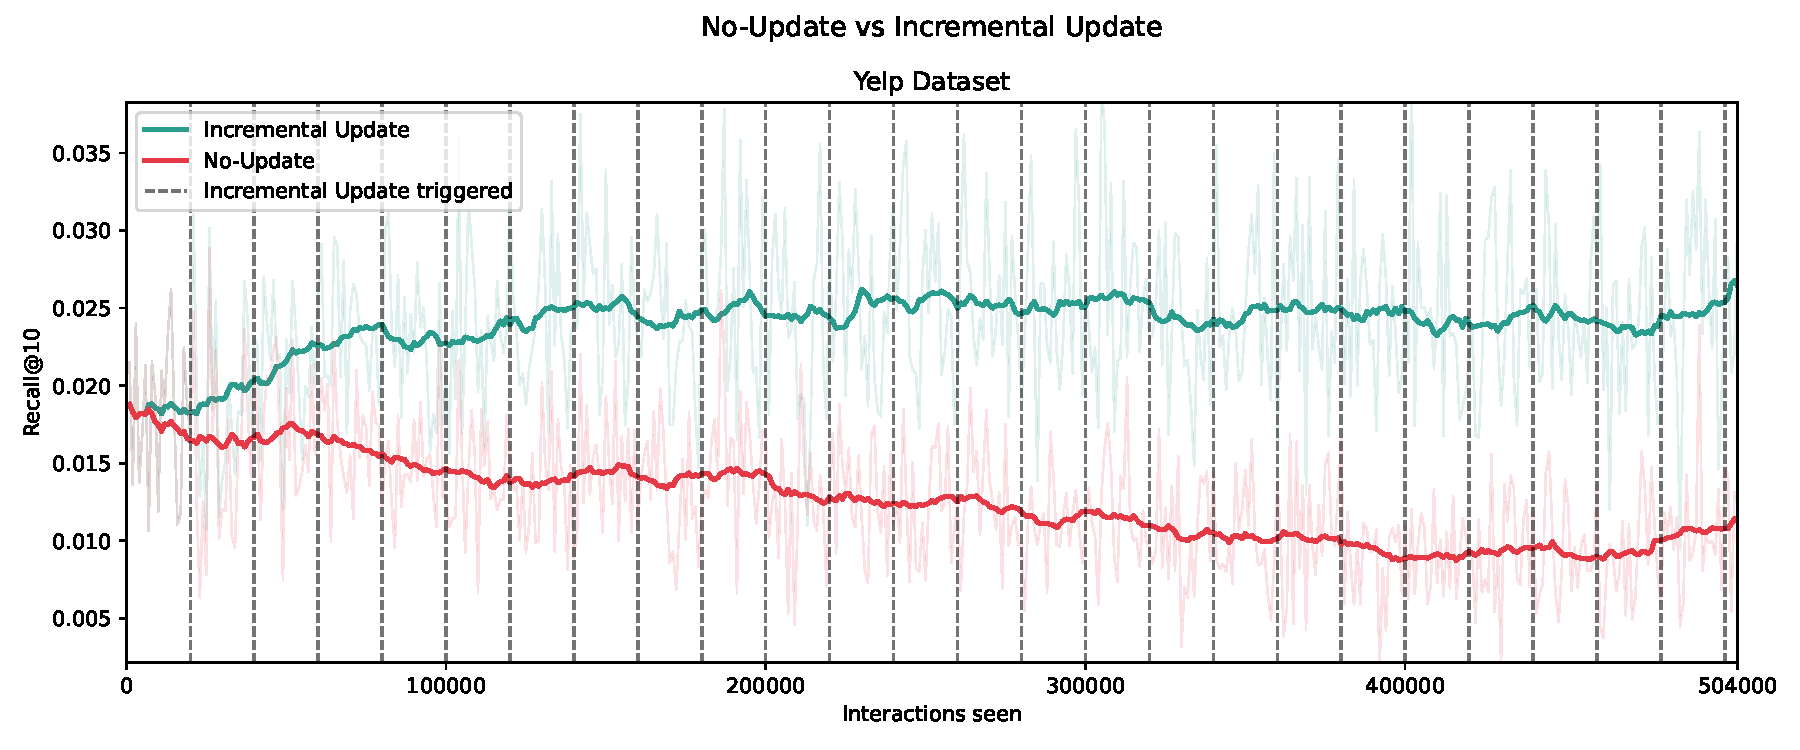
\includegraphics[width=0.95\linewidth]{yelptimecut_no_update_vs_incremental_recall_at_10.pdf}
    \end{figure}
\end{frame}


\begin{frame}{Yelp: Existing vs. New Users}
    \begin{figure}[h]
        \centering
        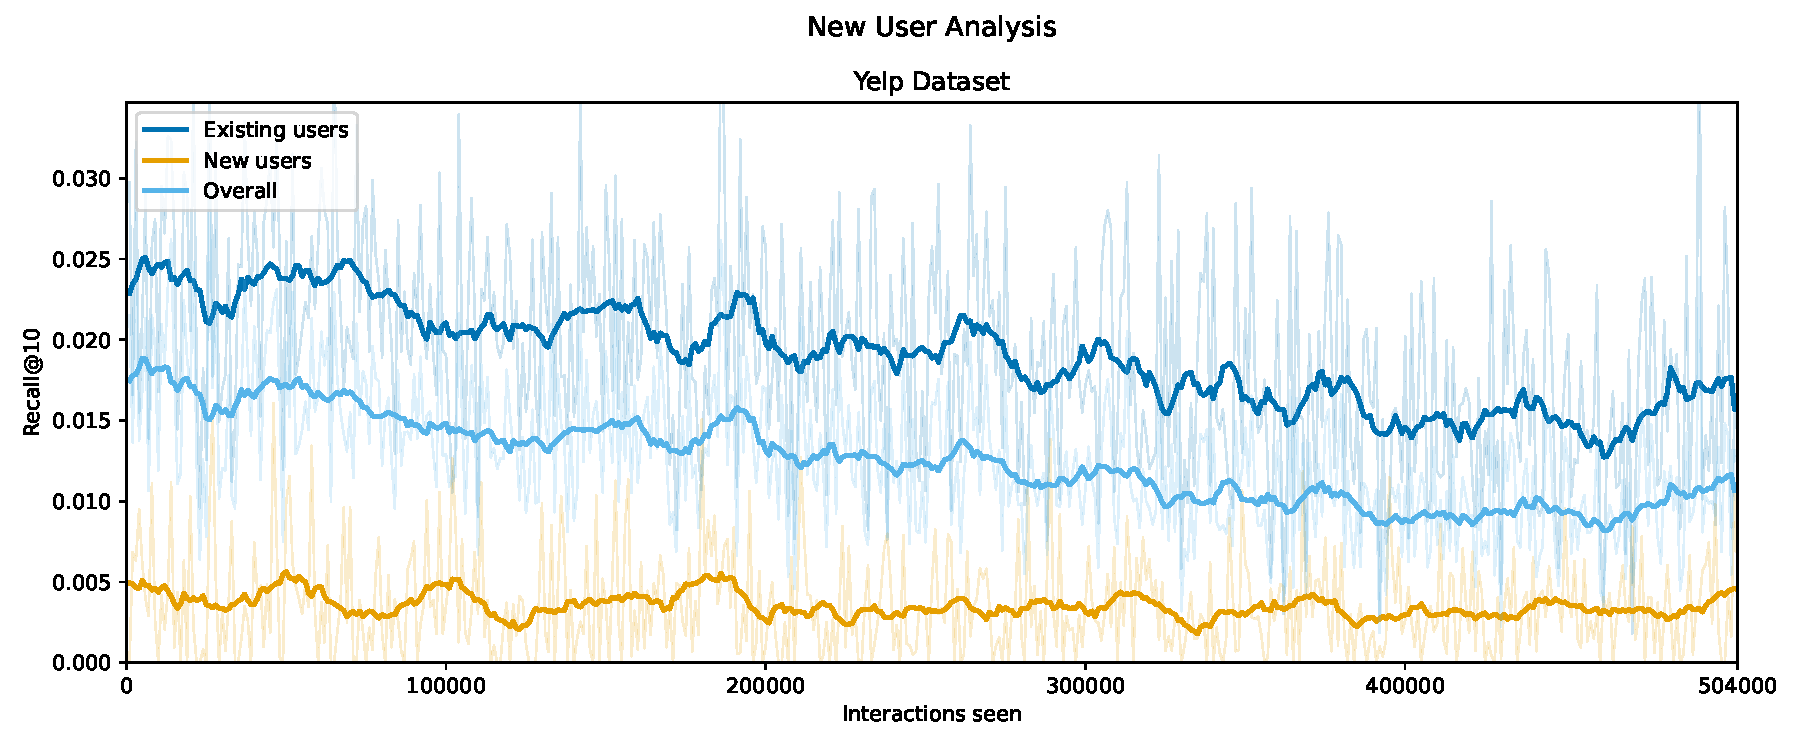
\includegraphics[width=0.95\linewidth]{yelptimecut_new_user_analysis_recall.pdf}
    \end{figure}
\end{frame}


\begin{frame}{Yelp: Content-Based Initialization}
    \begin{figure}[h]
        \centering
        \includegraphics<1>[width=0.95\linewidth]{yelptimecut_content_coldstart_vs_no_update_overall_recall.pdf}%
        \includegraphics<2>[width=0.95\linewidth]{yelptimecut_content_coldstart_vs_no_update_groups_recall.pdf}%
    \end{figure}
\end{frame}


\begin{frame}{Yelp: All Strategies}
    \begin{figure}[h]
        \centering
        \includegraphics<1>[width=0.95\linewidth]{yelptimecut_strategy_comparison_recall.pdf}%
        \includegraphics<2>[width=0.95\linewidth]{yelptimecut_content_init_vs_content_incremental_recall.pdf}%
    \end{figure}
\end{frame}


\begin{frame}{Comparison of Strategies}
    \Large
    \vspace*{\fill}
    \begin{table}[h]
\centering
\def\arraystretch{2}%  1 is the default, change whatever you need
\begin{tabular}{lcccc}
\toprule
& No-Update & Incremental & Content-Init & \makecell{Content +\\Incremental} \\
\midrule
Recall@10
& 0.0125
& \tikzmarkin<2>[hl]{a}(0.1,0.6)(0.1,-0.3) +91\% \tikzmarkend{a}
& \tikzmarkin<3>[hl]{b}(0.1,0.6)(0.1,-0.3) +41\% \tikzmarkend{b}
& \tikzmarkin<4>[hl]{c}(0.1,0.6)(0.1,-0.3) +106\% \tikzmarkend{c} \\
\makecell[l]{Emissions\\(\% of training)}
& 5.20\%
& \tikzmarkin<5>[hl]{d}(0.1,0.6)(0.1,-0.3) 6.82\%
& 6.14\%
& 7.55\% \tikzmarkend{d} \\
\bottomrule
\end{tabular}
\caption*{\large Mean Recall@10 (relative to no-update) and streaming emissions as a share of the one-time training cost on Yelp}
\end{table}
\end{frame}


\begin{frame}{Yelp: Update Frequency vs. Emissions}
    \begin{figure}[h]
        \centering
        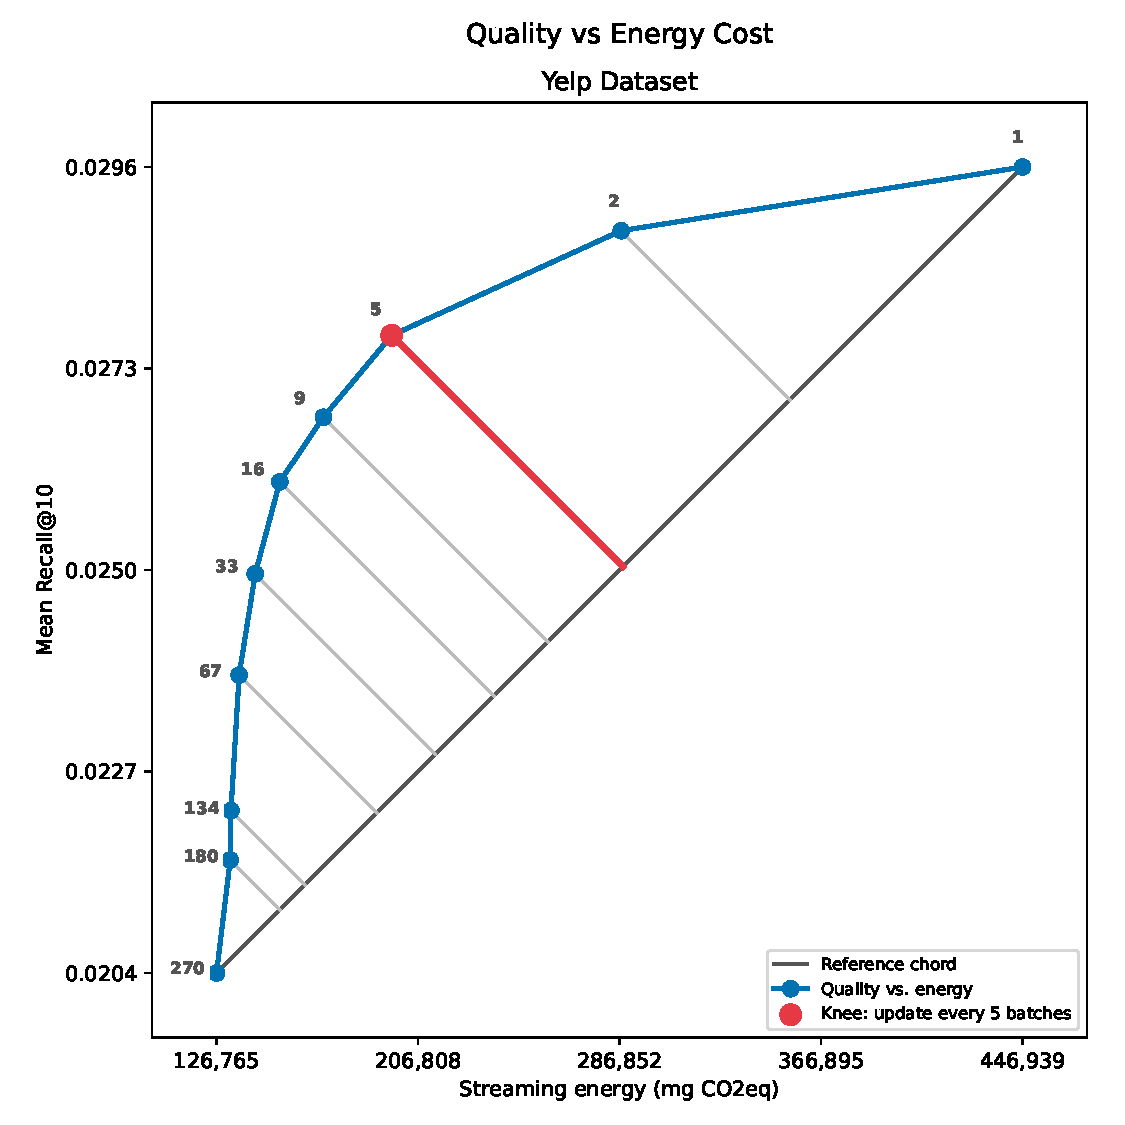
\includegraphics[width=0.42\linewidth]{yelptimecut_content_incremental_quality_vs_energy_recall.pdf}
    \end{figure}
    \footnotetext{\fullcite{satopaa2011kneedle}}
\end{frame}


\begin{frame}{MovieLens: All Strategies}
    \begin{figure}[h]
        \centering
        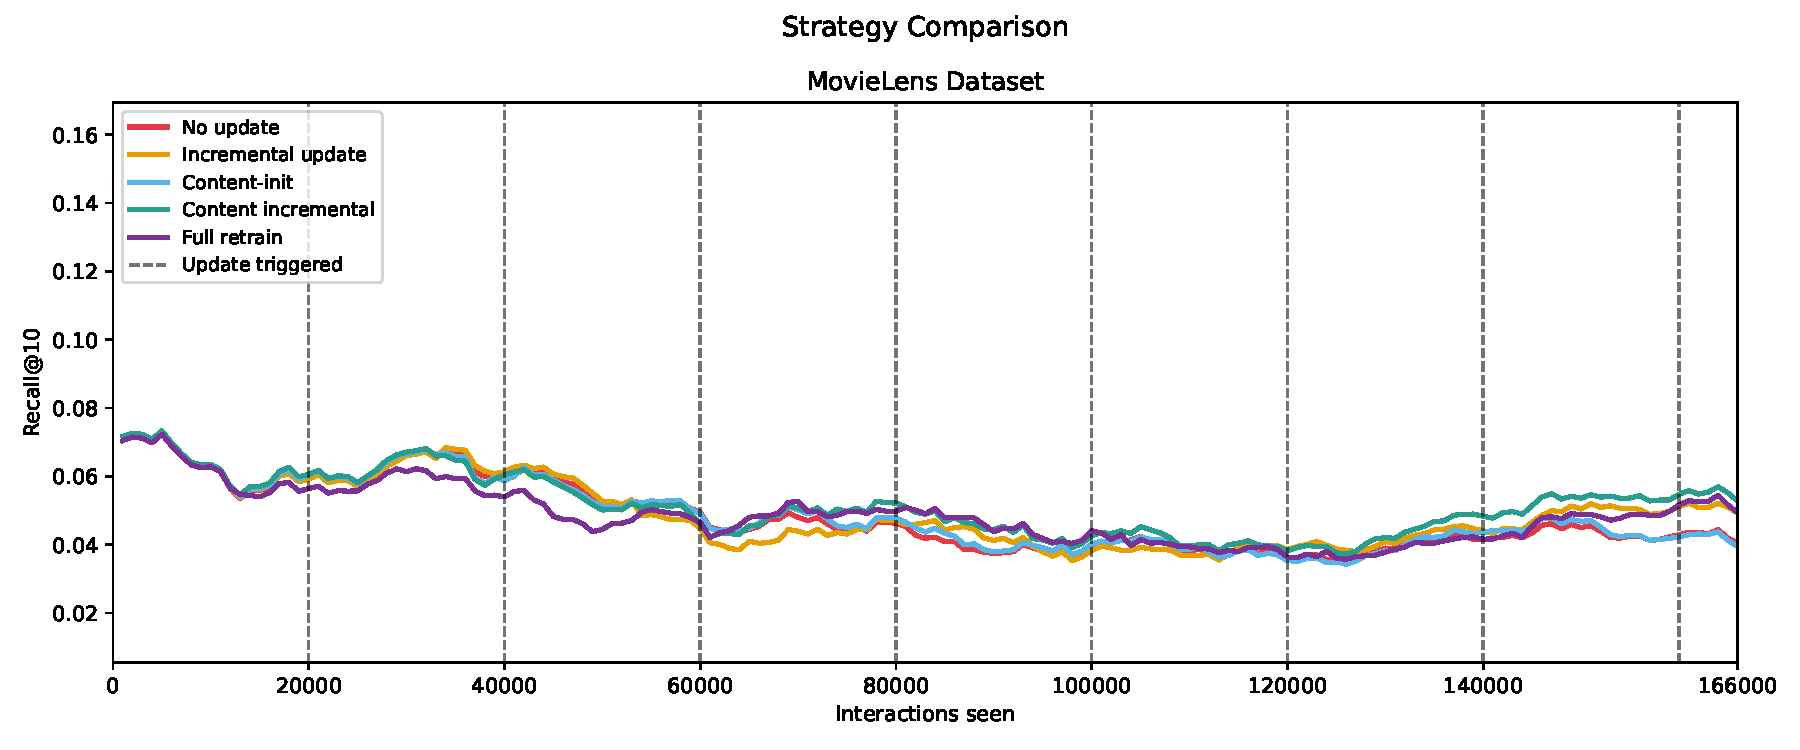
\includegraphics[width=0.95\linewidth]{ml1mtimecut_strategy_comparison_recall.pdf}
    \end{figure}
    \footnotetext{\fullcite{harper2015movielens}}
\end{frame}

% !TeX root = ../main.tex
% Add the above to each file to make compiling the PDF easier in some editors.

\section{Discussion}


\begin{frame}{Pitfall: Per-User Split}
    \begin{figure}[h]
        \centering
        \includegraphics<1>[width=0.95\linewidth]{yelp_strategy_comparison_recall.pdf}%
        \includegraphics<2>[width=0.95\linewidth]{yelptimecut_strategy_comparison_recall.pdf}%
    \end{figure}
    \footnotetext{\fullcite{ji2023leakage}}
\end{frame}


\begin{frame}{Conclusion}
    \setbeamercovered{transparent}
    \begin{center}
        \vspace{5mm}
        \Large Cheap updates recover most of the lost quality at a fraction of the training cost, but only where the data has something to correct\\
        \vspace{7mm}
        \pause
        \Huge$\Downarrow$\\
        \vspace{7mm}
        \LARGE Diagnose the source of decay before choosing an update strategy
    \end{center}
\end{frame}


\begin{frame}{Next Steps}
    \setbeamercovered{transparent}
    \begin{itemize}
        \large
        \setlength\itemsep{1.5em}
        \item Causal incremental graph convolution (CI-LightGCN), measured in energy rather than time\footnote{\fullcite{ding2022causal}}
        \pause
        \item Windowed graph construction to bound the update cost\footnote{\fullcite{ghiye2024rolling}}
        \pause
        \item Streams with controlled, documented drift\footnote{\fullcite{souza2020benchmarking}}
        \pause
        \item More datasets with less strict interaction filtering
    \end{itemize}
\end{frame}

% TODO: add more chapters here

% !TeX root = ../main.tex
% Add the above to each file to make compiling the PDF easier in some editors.

\begin{frame}{Acknowledgements}
    \vspace{4mm}
    \begin{center}
        \Huge \textcolor{TUMBlue}{Thank you!}
    \end{center}
    \begin{columns}
        \begin{column}{0.7\textwidth}
            \LARGE
            \vspace{2mm}\\
            \theChairName\\
            \vspace{5mm}
            Examiner: Prof. Dr.-Ing. Jörg Ott\\
            Advisor: Prof. Wolfgang Wörndl
        \end{column}
        \begin{column}{0.3\textwidth}
        \end{column}
    \end{columns}
\end{frame}

% !TeX root = ../main.tex
% Add the above to each file to make compiling the PDF easier in some editors.

\begin{frame}
    \vspace*{\fill}
    \begin{center}
        \Huge \textcolor{TUMBlue}{Appendix}
    \end{center}
\end{frame}

\appendix


\begin{frame}{Yelp: Precision@10, All Strategies}
    \begin{figure}[h]
        \centering
        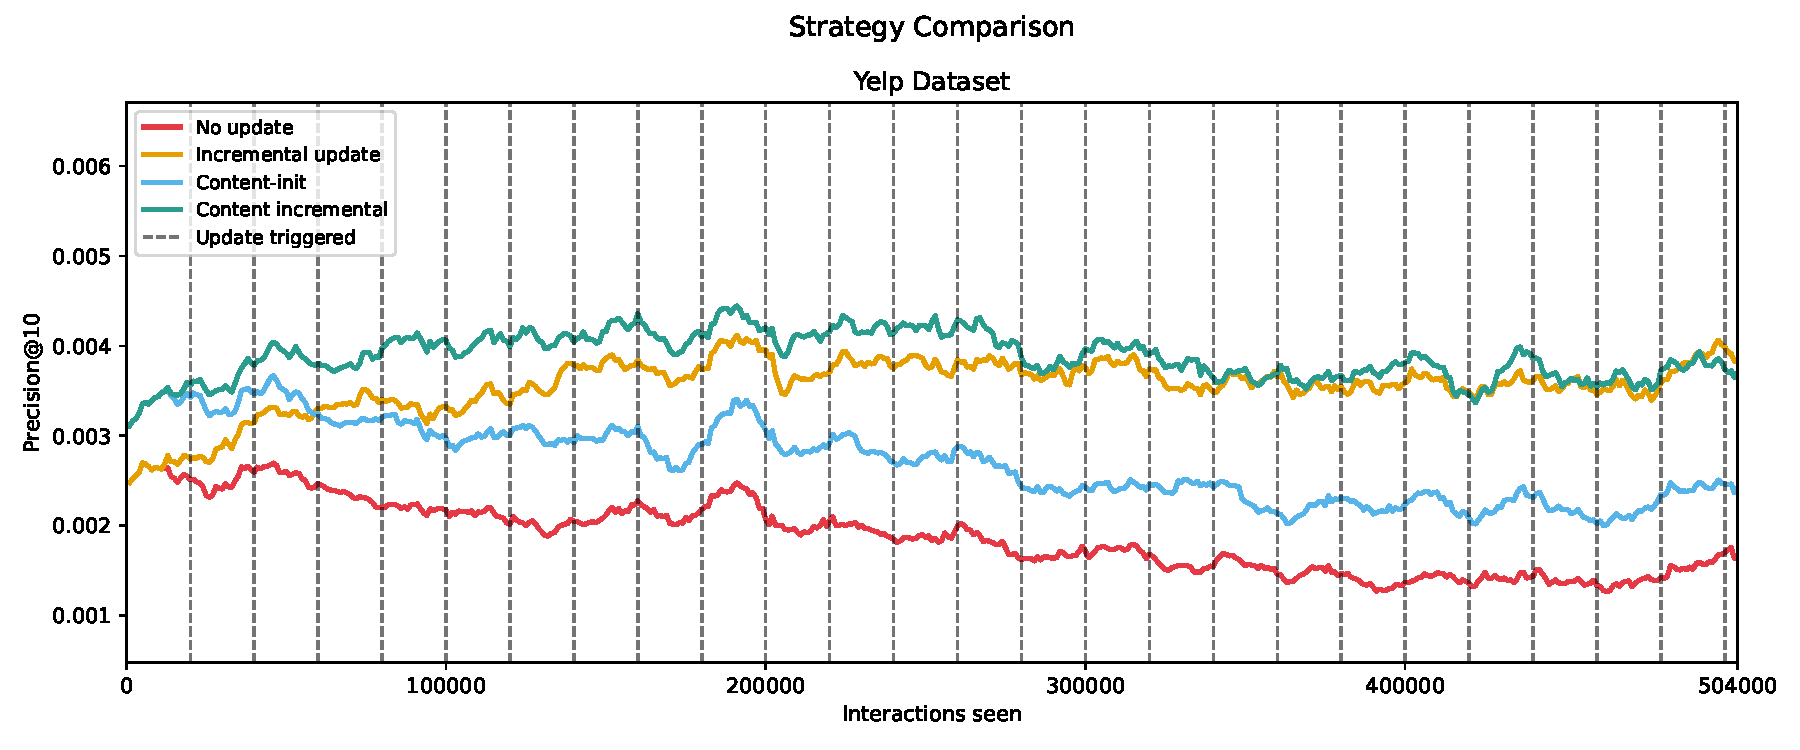
\includegraphics[width=0.95\linewidth]{yelptimecut_strategy_comparison_precision.pdf}
    \end{figure}
\end{frame}

\begin{frame}{Yelp: NDCG@10, All Strategies}
    \begin{figure}[h]
        \centering
        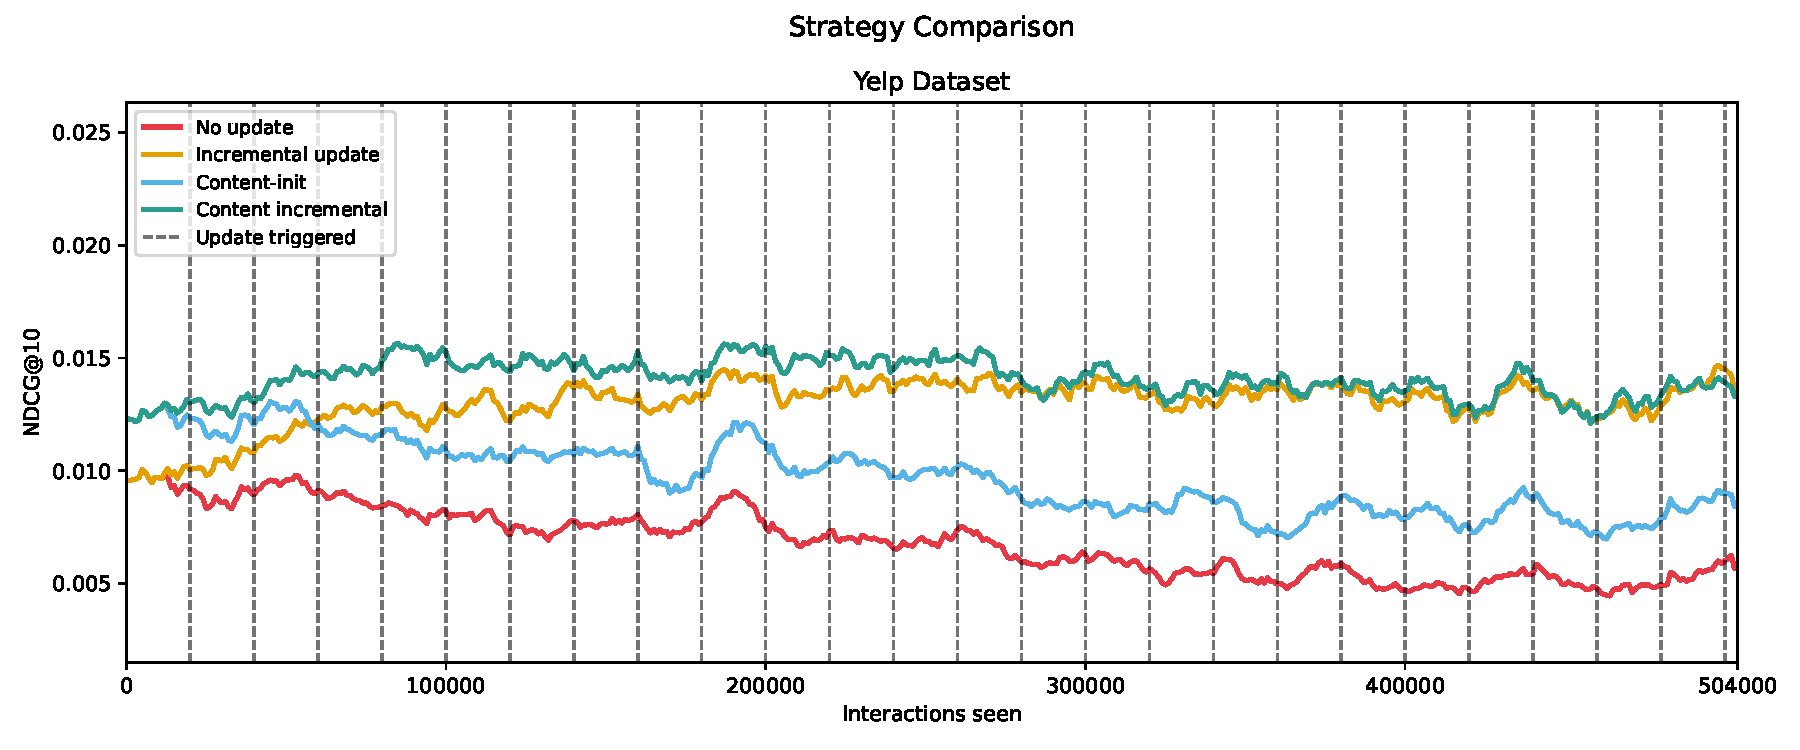
\includegraphics[width=0.95\linewidth]{yelptimecut_strategy_comparison_ndcg.pdf}
    \end{figure}
\end{frame}

\begin{frame}{Yelp: New Unique Users per Update Window}
    \begin{figure}[h]
        \centering
        \includegraphics<1>[width=0.95\linewidth]{yelptimecut_new_user_analysis_new_user_arrivals.pdf}%
        \includegraphics<2>[width=0.95\linewidth]{yelptimecutunfiltered_new_user_analysis_new_user_arrivals.pdf}%
    \end{figure}
\end{frame}

\begin{frame}{Yelp: Emissions by Phase}
    \begin{figure}[h]
        \centering
        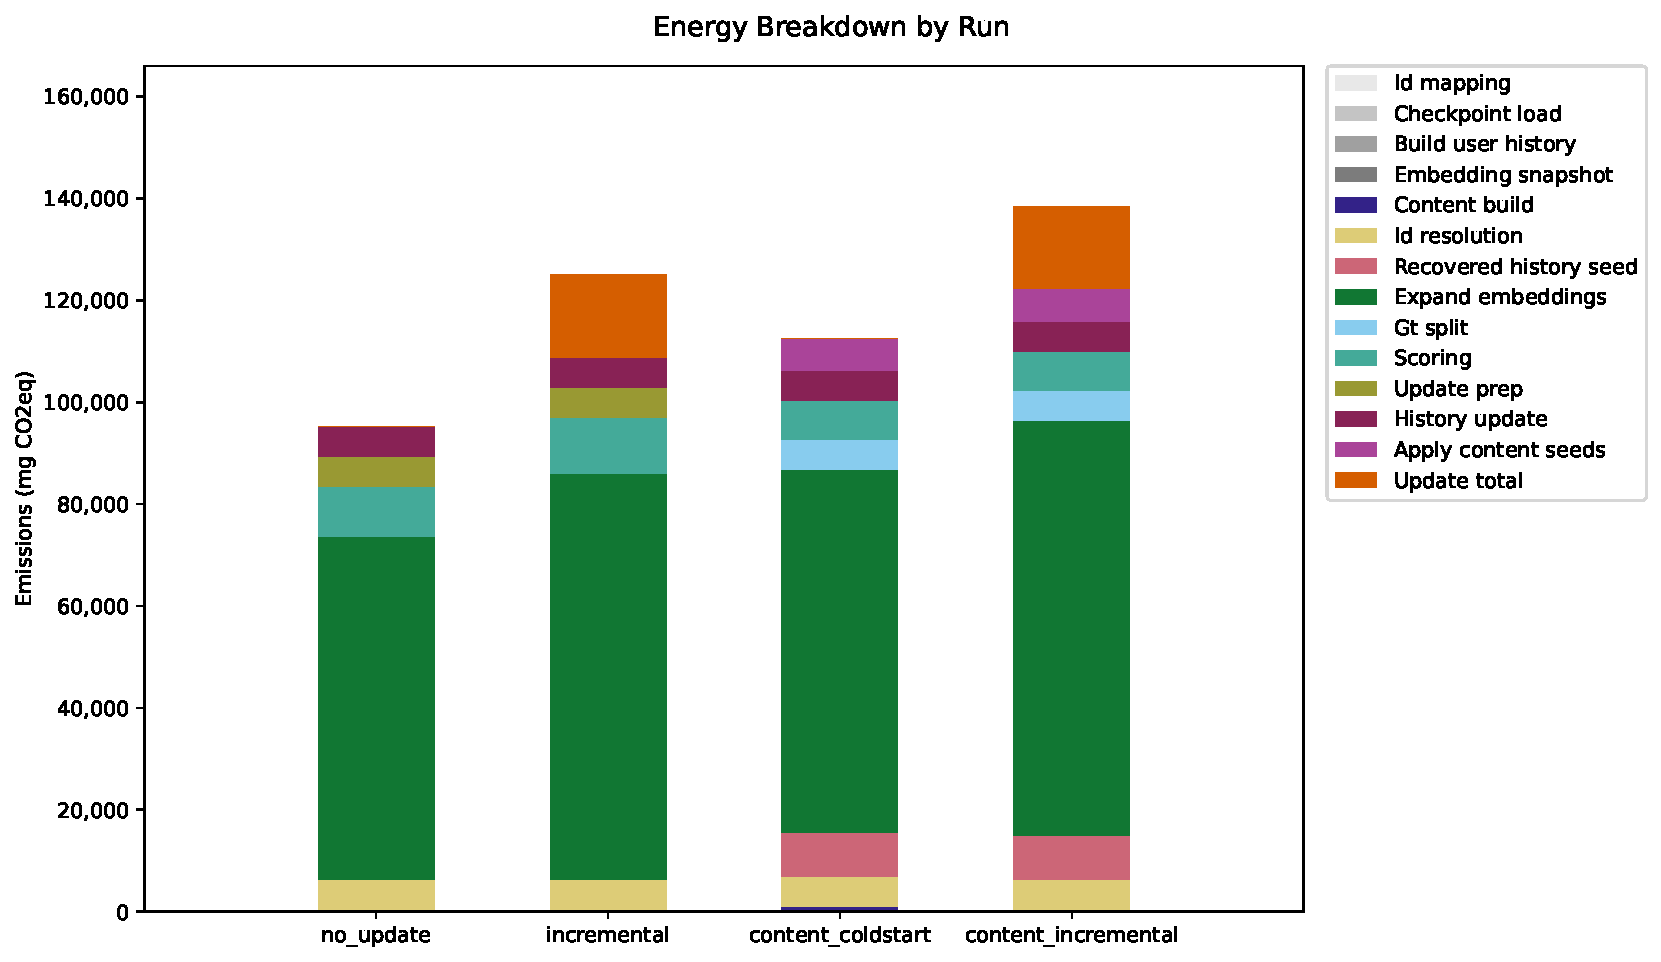
\includegraphics[width=0.7\linewidth]{yelptimecut_energy_summary_stacked.pdf}
    \end{figure}
\end{frame}

\begin{frame}{Yelp: Update Frequency Variants}
    \begin{figure}[h]
        \centering
        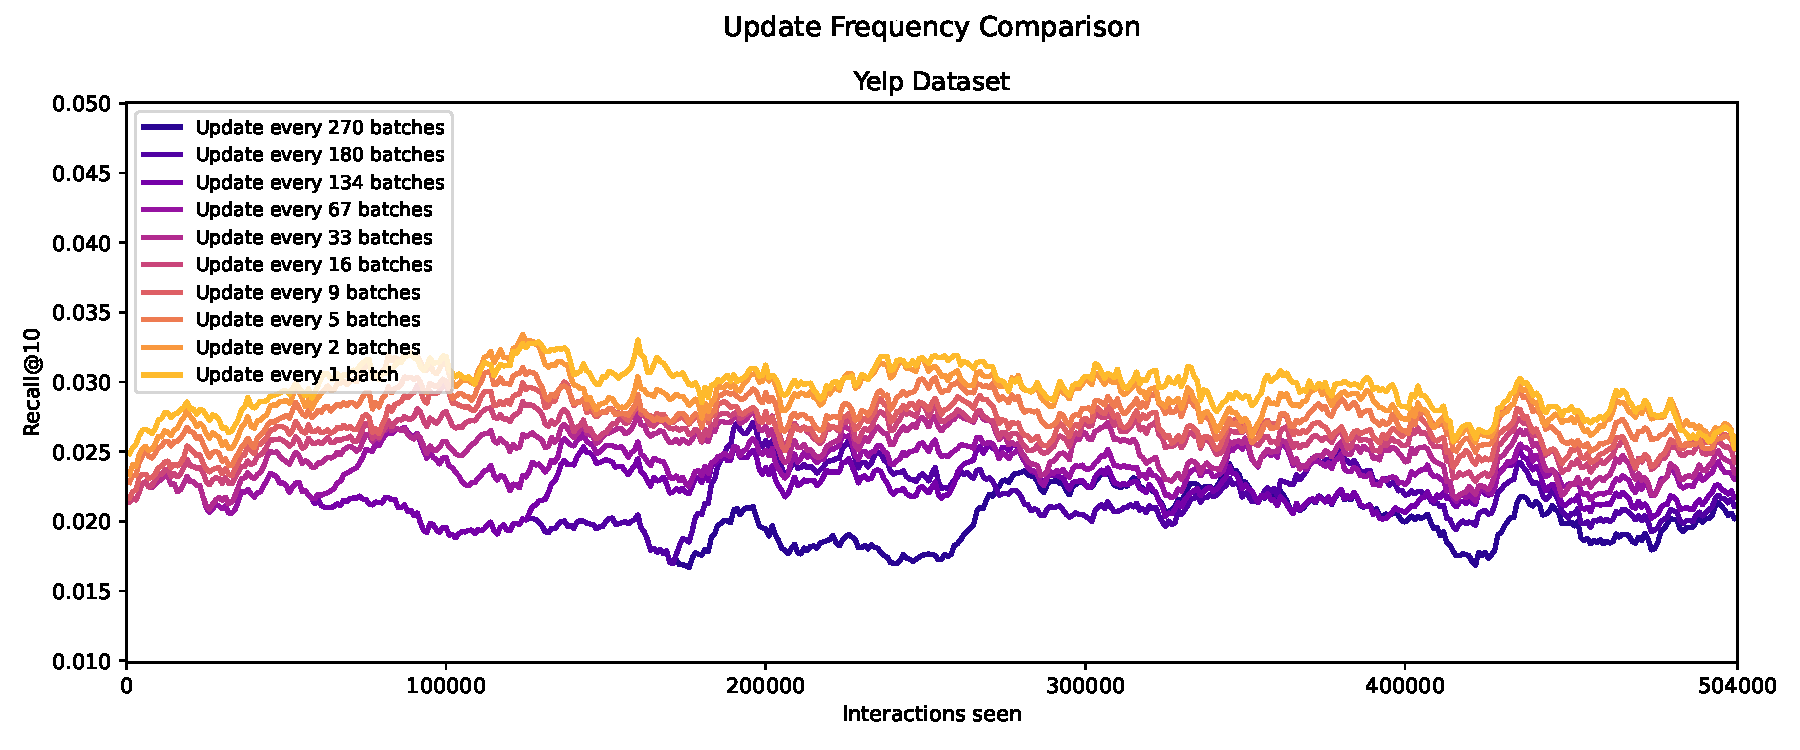
\includegraphics[width=0.95\linewidth]{yelptimecut_content_incremental_frequency_comparison_recall.pdf}
    \end{figure}
\end{frame}

\begin{frame}{Carbon Cost per Strategy}
    \begin{table}[h]
\centering
\def\arraystretch{1.6}%  1 is the default, change whatever you need
\begin{tabular}{lcccc}
\toprule
 & No-Update & Incremental & Content-Init & \makecell{Content +\\Incremental} \\
\midrule
Yelp streaming & 95{,}306 & 125{,}053 & 112{,}422 & 138{,}321 \\
Yelp training & \multicolumn{4}{c}{1{,}832{,}436} \\
MovieLens streaming & 17{,}286 & 18{,}654 & 20{,}045 & 22{,}618 \\
MovieLens training & \multicolumn{4}{c}{188{,}839} \\
\bottomrule
\end{tabular}
\caption*{Carbon emissions in mg CO$_2$eq. Full retrain on MovieLens: 1{,}387{,}568 streaming, $792\times$ incremental per update.}
\end{table}
\end{frame}


\begin{frame}[allowframebreaks]{References}
    \scriptsize
    \printbibliography[heading=none]
\end{frame}


\end{document}
